\chapter{Counting Like a Computer}
\label{countingchapter}

%  FIXME - See Dominique note 

% 
% 
% Copyright 2002 Jonathan Bartlett
% 
% Permission is granted to copy, distribute and/or modify this
% document under the terms of the GNU Free Documentation License,
% Version 1.1 or any later version published by the Free Software
% Foundation; with no Invariant Sections, with no Front-Cover Texts,
% and with no Back-Cover Texts.  A copy of the license is included in fdl.xml
% 

\section{Counting}

\section{Counting Like a Human}

In many ways, computers count just like humans.  So, before we
start learning how computers count, let's take a deeper look at
how we count.

How many fingers do you have?  No, it's not a trick question.
Humans (normally) have ten fingers.  Why is that significant?
Look at our numbering system.  At what point does a one-digit
number become a two-digit number?  That's right, at ten.  Humans
count and do math using a base ten numbering system.  Base ten
means that we group everything in tens.  Let's say we're counting
sheep.  1, 2, 3, 4, 5, 6, 7, 8, 9, 10.  Why did we all of a sudden
now have two digits, and re-use the 1?  That's because we're grouping
our numbers by ten, and we have 1 group of ten sheep.  Okay, let's
go to the next number 11.  That means we have 1 group of ten sheep,
and 1 sheep left ungrouped.  So we continue - 12, 13, 14, 15, 16, 17,
18, 19, 20.  Now we have 2 groups of ten.  21 - 2 groups of ten, and
1 sheep ungrouped.  22 - 2 groups of ten, and 2 sheep ungrouped.   So,
let's say we keep counting, and get to 97, 98, 99, and 100.  Look, it
happened again!  What happens at 100?  We now have ten groups of ten.
At 101 we have ten groups of ten, and 1 ungrouped sheep.  So we can
look at any number like this.  If we counted 60879 sheep, that would
mean that we had 6 groups of ten groups of ten groups of ten groups of ten,
0 groups of ten groups of ten groups of ten, 8 groups of ten groups of ten,
7 groups of ten, and 9 sheep left ungrouped.  

So, is there anything significant about grouping things by ten?  No!  It's
just that grouping by ten is how we've always done it, because we have
ten fingers.  We could have grouped at nine or at eleven (in which case
we would have had to make up a new symbol).  The only difference between
the different groupings of numbers is that we have to re-learn our
multiplication, addition, subtraction, and division tables for each
grouping.  The rules
haven't changed, just the way we represent them.  Also, some of our
tricks that we learned don't always apply, either.  For example, let's
say we grouped by nine instead of ten.  Moving the decimal point one
digit to the right no longer multiplies by ten, it now multiplies by nine.
In base nine, 500 is only nine times as large as 50.

\section{Counting Like a Computer}

The question is, how many fingers does the computer have to count with?
The computer only has two fingers.  So that means all of the groups are 
groups of two.  So, let's count in binary - 0 (zero), 1 (one), 10 (two - 
one group of two), 11 (three - one group of two and one left over), 
100 (four - two groups of two), 101 (five - two groups of two and one left 
over), 110 (six - two groups of two and one group of two), and so on.  
In base two, moving the decimal one digit to the right multiplies by two, and 
moving it to the left divides by two.  Base two\index{base two} is also referred to
as binary.

The nice thing about base two is that the basic math tables are very
short.  In base ten, the multiplication tables are ten columns wide,
and ten columns tall.  In base two, it is very simple:

\begin{simpletyping}
\begin{lstlisting}
%  NOTE - these need to be converted to tables 

Table of binary addition

+ |  0  |  1  
--+-----+-----
0 |  0  |  0  
--+-----+-----
1 |  1  | 10  

Table of binary multiplication

* |  0  |  1
--+-----+-----
0 |  0  |  0
--+-----+-----
1 |  0  |  1

\end{lstlisting}
\end{simpletyping}

So, let's add the numbers 10010101 with 1100101:

\begin{simpletyping}
\begin{lstlisting}
   10010101
+   1100101
-----------
   11111010
\end{lstlisting}
\end{simpletyping}

Now, let's multiply them:

\begin{simpletyping}
\begin{lstlisting}

        10010101
     *   1100101
     -----------
        10010101
       00000000
      10010101
     00000000
    00000000
   10010101
  10010101
 ---------------
  11101011001001
\end{lstlisting}
\end{simpletyping}

\section{Conversions Between Binary and Decimal}

Let's learn how to convert numbers from binary\index{binary} (base two\index{base two}) to 
decimal\index{decimal} (base ten\index{base ten}).  This is actually a rather simple process.
If you remember, each digit\index{digit} stands for some grouping of two.  So,
we just need to add up what each digit represents, and we will have
a decimal number.  Take the binary number 10010101.  To find out
what it is in decimal, we take it apart like this:

\begin{simpletyping}
\begin{lstlisting}
     1    0    0    1    0    1    0    1
     |    |    |    |    |    |    |    |
     |    |    |    |    |    |    |    Individual units (2\textasciicircum 0)
     |    |    |    |    |    |    0 groups of 2 (2\textasciicircum 1)
     |    |    |    |    |    1 group of 4 (2\textasciicircum 2)
     |    |    |    |    0 groups of 8 (2\textasciicircum 3)
     |    |    |    1 group of 16 (2\textasciicircum 4)
     |    |    0 groups of 32 (2\textasciicircum 5)
     |    0 groups of 64 (2\textasciicircum 6)
     1 group of 128 (2\textasciicircum 7)
\end{lstlisting}
\end{simpletyping}

and then we add all of the pieces together, like this:

\begin{simpletyping}
\begin{lstlisting}
1*128 + 0*64 + 0*32 + 1*16 + 0*8 + 1*4 + 0*2 + 1*1 =
128 + 16 + 4 + 1 = 
149
\end{lstlisting}
\end{simpletyping}

So 10010101 in binary is 149 in decimal.  Let's look at 1100101.  It
can be written as

\begin{simpletyping}
\begin{lstlisting}
1*64 + 1*32 + 0 * 16 + 0*8 + 1*4 + 0*2 + 1*1 =
64 + 32 + 4 + 1 =
101
\end{lstlisting}
\end{simpletyping}

So we see that 1100101 in binary is 101 in decimal.  Let's look at
one more number, 11101011001001.  You can convert it to decimal by doing

\begin{simpletyping}
\begin{lstlisting}
1*8192 + 1*4096 + 1*2048 + 0*1024 + 1*512 + 0*256 
       + 1*128 + 1*64 + 0*32 + 0*16 + 1*8 + 0*4 
       + 0*2 + 1*1 =

8192 + 4096 + 2048 + 512 + 128 + 64 + 8 + 1 =

15049
\end{lstlisting}
\end{simpletyping}

Now, if you've been paying attention, you have noticed that the numbers
we just converted are the same ones we used to multiply with earlier.
So, let's check our results: 101 * 149 = 15049.  It worked!

Now let's look at going from decimal\index{decimal} back to binary\index{binary}.  In order to do
the conversion, you have to \emph{divide} the number
into groups of two.  So, let's say you had the number 17.  If you
divide it by two, you get 8 with 1 left over.  So that means there are
8 groups of two, and 1 ungrouped.  That means that the rightmost digit
will be 1.  Now, we have the rigtmost digit figured out, and 8 groups
of 2 left over.  Now, let's see how many groups of two groups of two we 
have, by dividing 8 by 2.  We get 4, with nothing left over.  That
means that all groups two can be further divided into more groups of
two.  So, we have 0 groups of only two.  So the next digit to the
left is 0.  So, we divide 4 by 2 and get two, with 0 left over, so
the next digit is 0.  Then, we divide 2 by 2 and get 1, with 0 left over.
So the next digit is 0.  Finally, we divide 1 by 2 and get 0 with 1
left over, so the next digit to the left is 1.  Now, there's nothing
left, so we're done.  So, the number we wound up with is 10001.

Previously, we converted to binary 11101011001001 to decimal 15049.  Let's
do the reverse to make sure that we did it right:

\begin{simpletyping}
\begin{lstlisting}
15049 / 2 = 7524    Remaining 1
7524 / 2 = 3762     Remaining 0
3762 / 2 = 1881     Remaining 0
1881 / 2 = 940      Remaining 1
940 / 2 = 470       Remaining 0
470 / 2 = 235       Remaining 0
235 / 2 = 117       Remaining 1
117 / 2 = 58        Remaining 1
58 / 2 = 29         Remaining 0
29 / 2 = 14         Remaining 1
14 / 2 = 7          Remaining 0
7 / 2 = 3           Remaining 1
3 / 2 = 1           Remaining 1
1 / 2 = 0           Remaining 1
\end{lstlisting}
\end{simpletyping}

Then, we put the remaining numbers back together, and we have the original
number!  Remember the first division remainder goes to the far right, so
from the bottom up you have 11101011001001.

Each digit in a binary number is called a \emph{bit\index{bits}}, which
stands for \emph{binary digit\index{binary digit}}.  Remember, computers divide up
their memory into storage locations called bytes\index{bytes}.  Each storage location on an x86 processor (and most others) is 8 bits long.  Earlier we said
that a byte can hold any number between 0 and 255.  The reason for this
is that the largest number you can fit into 8 bits is 255.  You can
see this for yourself if you convert binary 11111111 into decimal:

\begin{simpletyping}
\begin{lstlisting}
11111111 =

(1 * 2\textasciicircum 7) + (1 * 2\textasciicircum 6) + (1 * 2\textasciicircum 5) + (1 * 2\textasciicircum 4) + (1 * 2\textasciicircum 3) 
          + (1 * 2\textasciicircum 2) + (1 * 2\textasciicircum 1) + (1 * 2\textasciicircum 0) = 

128 + 64 + 32 + 16 + 8 + 4 + 2 + 1 =

255
\end{lstlisting}
\end{simpletyping}

The largest number that you can hold in 16 bits is 65535.   The largest
number you can hold in 32 bits is 4294967295 (4 billion).  The largest
number you can hold in 64 bits is 18,446,744,073,709,551,615.  The
largest number you can hold in 128 bits is
340,282,366,920,938,463,463,374,607,431,768,211,456.  Anyway, you
see the picture.  For x86 processors, most of the time you will deal with 4-byte
numbers (32 bits), because that's the size of the registers\index{registers}.

\section{Truth, Falsehood, and Binary Numbers}
\label{truthbinarynumbers}

Now we've seen that the computer stores everything as sequences of
1's and 0's.  Let's look at some other uses of this.  What if, instead
of looking at a sequence of bits\index{bits} as a number, we instead looked at
it as a set of switches\index{switches}.  For example, let's say there are four switches
that control lighting in the house.  We have a switch for outside lights,
a switch for the hallway lights, a switch for the living room lights,
and a switch for the bedroom lights.  We could make a little table
showing which of these were on and off, like so:

\begin{simpletyping}
\begin{lstlisting}
Outside  Hallway  Living Room  Bedroom
  On       Off        On         On
\end{lstlisting}
\end{simpletyping}

It's obvious from looking at this that all of the lights are on except
the hallway ones.  Now, instead of using the words "On" and "Off",
let's use the numbers 1 and 0.  1 will represent on, and 0 will represent
off.  So, we could represent the same information as

\begin{simpletyping}
\begin{lstlisting}
Outside  Hallway  Living Room  Bedroom
   1        0           1         1
\end{lstlisting}
\end{simpletyping}

Now, instead of having labels on the light switches, let's say we just
memorized which position went with which switch.  Then, the same
information could be represented as

\begin{simpletyping}
\begin{lstlisting}
1           0           1         1
\end{lstlisting}
\end{simpletyping}

or as

\begin{simpletyping}
\begin{lstlisting}
1011
\end{lstlisting}
\end{simpletyping}

This is just one of many ways you can use the computers storage locations
to represent more than just numbers.  The computers memory just sees numbers,
but programmers can use these numbers to represent anything their imaginations
can come up with.  They just sometimes have to be creative when figuring out
the best representation.

Not only can you do regular arithmetic with binary numbers, they also have
a few operations of their own, called binary
\index{binary operations} 
or logical operations
\index{logical operations}.  
The standard binary operations are

\begin{itemize}\item AND\index{AND} 
\item OR\index{OR} 
\item NOT\index{NOT} 
\item XOR\index{XOR} 
\end{itemize}

Before we look at examples, I'll describe them for you.
AND takes two bits and returns one bit.  AND will return a 1 only if
both bits are 1, and a 0 otherwise.  For example, 1 AND 1 is 1, but
1 AND 0 is 0, 0 AND 1 is 0, and 0 AND 0 is 0.  

OR takes two bits
and returns one bit.  It will return 1 if either of the original bits
is 1.  For example, 1 OR 1 is 1, 1 OR 0 is one, 0 OR 1 is 1, but 0 OR 0
is 0.

NOT only takes one bit and returns its opposite.  NOT 1 is 0 and
NOT 0 is 1.  

Finally, XOR is like OR, except it returns 0 if both bits
are 1.

Computers can do these operations on whole registers at a time.
For example, if a register has 10100010101010010101101100101010 and
another one has 10001000010101010101010101111010, you can run any of
these operations on the whole registers.  For example, if we were to
AND them, the computer will run from the first bit to the 32nd and run
the AND\index{AND} operation on that bit in both registers.  In this case:

\begin{simpletyping}
\begin{lstlisting}
10100010101010010101101100101010 AND
10001000010101010101010101111010
--------------------------------
10000000000000010101000100101010
\end{lstlisting}
\end{simpletyping}

You'll see that the resulting set of bits only has a one where 
\emph{both} numbers had a one, and in every other position
it has a zero.  Let's look at what an OR\index{OR} looks like:

\begin{simpletyping}
\begin{lstlisting}
10100010101010010101101100101010 OR 
10001000010101010101010101111010
--------------------------------
10101010111111010101111101111010
\end{lstlisting}
\end{simpletyping}

In this case, the resulting number has a 1 where either number has
a 1 in the given position.  Let's look at the NOT\index{NOT} operation:

\begin{simpletyping}
\begin{lstlisting}
NOT 10100010101010010101101100101010
------------------------------------
    01011101010101101010010011010101
\end{lstlisting}
\end{simpletyping}

This just reverses each digit.  Finally, we have XOR\index{XOR}, which is
like an OR, except if \emph{both} digits are 1, it
returns 0.

\begin{simpletyping}
\begin{lstlisting}
10100010101010010101101100101010 XOR 
10001000010101010101010101111010
--------------------------------
00101010111111000000111001010000
\end{lstlisting}
\end{simpletyping}

This is the same two numbers used in the OR operation, so you can 
compare how they work.  Also, if you XOR a number with itself, you 
will always get 0, like this:

\begin{simpletyping}
\begin{lstlisting}
10100010101010010101101100101010 XOR 
10100010101010010101101100101010
--------------------------------
00000000000000000000000000000000
\end{lstlisting}
\end{simpletyping}

These operations are useful for two reasons:

\begin{itemize}\item The computer can do them extremely fast 
\item You can use them to compare many truth values at the same time 
\end{itemize}

You may not have known that different instructions execute at different
speeds.  It's true, they do.  And these operations are the
fastest on most processors.  For example, you saw that XORing a number with 
itself produces 0.  Well, the XOR\index{XOR} operation is faster than the loading operation, so
many programmers use it to load a register\index{register} with zero.  For example, the
code

\begin{simpletyping}
\begin{lstlisting}
	movl  \$0, {\eaxBare}
\end{lstlisting}
\end{simpletyping}

is often replaced by

\begin{simpletyping}
\begin{lstlisting}
	xorl  {\eaxBare}, {\eaxBare}
\end{lstlisting}
\end{simpletyping}

We'll discuss speed more in \autoref{optimizationch}, but I want you
to see how programmers often do tricky things, especially with these
binary operators, to make things fast.  Now let's look at how we
can use these operators to manipulate true\index{true}/false\index{false} values.  Earlier
we discussed how binary numbers can be used to represent any number
of things.  Let's use binary numbers to represent what things my
Dad and I like.  First, let's look at the things I like:

\begin{simpletyping}
\begin{lstlisting}
Food: yes
Heavy Metal Music: yes
Wearing Dressy Clothes: no
Football: yes
\end{lstlisting}
\end{simpletyping}

Now, let's look at what my Dad likes:

\begin{simpletyping}
\begin{lstlisting}
Food: yes
Heavy Metal Music: no
Wearing Dressy Clothes: yes
Football: yes
\end{lstlisting}
\end{simpletyping}

Now, let's use a 1 to say yes we like something, and a 0 to say no we don't.
Now we have:

\begin{simpletyping}
\begin{lstlisting}
Me
Food: 1
Heavy Metal Music: 1
Wearing Dressy Clothes: 0
Football: 1

Dad
Food: 1
Heavy Metal Music: 0
Wearing Dressy Clothes: 1
Football: 1
\end{lstlisting}
\end{simpletyping}

Now, if we just memorize which position each of these are in, we have

\begin{simpletyping}
\begin{lstlisting}
Me
1101

Dad
1011
\end{lstlisting}
\end{simpletyping}

Now, let's see we want to get a list of things both my Dad and I like.
You would use the AND\index{AND} operation.  So

\begin{simpletyping}
\begin{lstlisting}
1101 AND
1011
--------
1001
\end{lstlisting}
\end{simpletyping}

Which translates to

\begin{simpletyping}
\begin{lstlisting}
Things we both like
Food: yes
Heavy Metal Music: no
Wearing Dressy Clothes: no
Football: yes
\end{lstlisting}
\end{simpletyping}

Remember, the computer has no idea what the ones and zeroes represent.
That's your job and your program's job.  If you wrote a program
around this representation your program would at some point examine
each bit and have code to tell the user what it's for (if you asked a computer
what two people agreed on and it answered 1001, it wouldn't be very
useful).  Anyway, let's say we want to know the things that we disagree
on.  For that we would use XOR\index{XOR}, because it will return 1 only if one
or the other is 1, but not both.  So

\begin{simpletyping}
\begin{lstlisting}
1101 XOR
1011
--------
0110
\end{lstlisting}
\end{simpletyping}

And I'll let you translate that back out.  

The previous operations: AND, OR, NOT, and XOR are called 
\emph{boolean operators\index{boolean operators}} 
because they were first studied by George Boole.  
So, if someone mentiones boolean operators\index{boolean operators} or 
boolean algebra\index{boolean algebra}, 
you now know what they are talking about.

In addition to the boolean operations, there
are also two binary operators\index{binary operators} that aren't boolean, shift\index{shift} and rotate\index{rotate}.
Shifts and rotates each do what their name implies, and can do so to
the right or the left.  A left shift moves each digit of a binary number
one space to the left, puts a zero in the ones spot, and chops off
the furthest digit to the left.  A left rotate does the same thing, but
takes the furthest digit to the left and puts it in the ones spot.  For
example,

\begin{simpletyping}
\begin{lstlisting}
Shift left  10010111 = 00101110
Rotate left 10010111 = 00101111
\end{lstlisting}
\end{simpletyping}

Notice that if you rotate a number for every digit it has (i.e. - rotating a 32-bit number 32 times), you wind up
with the same number you started with.  However, if you \emph{shift} a number for every digit 
you have, you wind up with 0.  So, what are these shifts useful for?
Well, if you have binary numbers representing things, you use shifts
to peek at each individual value.  Let's say, for instance, that
we had my Dad's likes stored in a register (32 bits).  It
would look like this:

\begin{simpletyping}
\begin{lstlisting}
00000000000000000000000000001011
\end{lstlisting}
\end{simpletyping}

Now, as we said previously, this doesn't work as program output.  So,
in order to do output, we would need to do shifting\index{shifting} and 
\emph{masking\index{masking}}.  Masking is the process of eliminating
everything you don't want.  In this case, for every value we are looking
for, we will shift the number so that value is in the ones place, and
then mask that digit so that it is all we see.  Masking is accomplished
by doing an AND\index{AND} 
with a number that has the bits we are interested in set to 1.
For example, let's say
we wanted to print out whether my Dad likes dressy clothes or not.  That
data is the second value from the right.  So, we have to shift the
number right 1 digit so it looks like this:

\begin{simpletyping}
\begin{lstlisting}
00000000000000000000000000000101
\end{lstlisting}
\end{simpletyping}

and then, we just want to look at that digit, so we mask it by ANDing
it with 00000000000000000000000000000001.

\begin{simpletyping}
\begin{lstlisting}
00000000000000000000000000000101 AND
00000000000000000000000000000001
-----------------------------------
00000000000000000000000000000001
\end{lstlisting}
\end{simpletyping}

This will make the value of the register 1 if my Dad likes dressy
clothes, and 0 if he doesn't.  Then we can do a comparison to 1
and print the results.  The code would look like this:

\begin{simpletyping}
\begin{lstlisting}
	\#NOTE - assume that the register {\ebxBare} holds 
	\#       my Dad's preferences

	movl  {\ebxBare}, {\eaxBare} \#This copies the information into {\eaxBare} so
	                 \#we don't lose the original data

	shrl  \$1, {\eaxBare}   \#This is the shift operator.  It stands
	                 \#for Shift Right Long.  This first number
	                 \#is the number of positions to shift,
	                 \#and the second is the register to shift
	
	\#This does the masking
	andl  \$0b00000000000000000000000000000001, {\eaxBare} 

	\#Check to see if the result is 1 or 0
	cmpl  \$0b00000000000000000000000000000001, {\eaxBare} 

	je    yes\_he\_likes\_dressy\_clothes

	jmp   no\_he\_doesnt\_like\_dressy\_clothes
\end{lstlisting}
\end{simpletyping}

And then we would have two labels which printed something about
whether or not he likes dressy clothes and then exits.
The \icode{0b} notation means that what follows is a binary number\index{binary number}.  
In this case it wasn't needed, because 1 is the same in any
numbering system, but I put it there for clarity.  
We also didn't need the 31 zeroes, but I put them in
to make a point that the number you are using is 32 bits.

When a number represents a set of options for a function\index{functions} or system call\index{system call},
the individual true/false elements are called \emph{flags\index{flags}}.
Many system calls have numerous options that are all
set in the same register using a mechanism like we've described.
The \icode{open\index{open}} system call, for example, has as its
second parameter a list of flags to tell the operating system how
to open the file.  Some of the flags include:

\begin{description}

\item[\icode{O\_WRONLY\index{O\_WRONLY}}] This flag is \icode{0b00000000000000000000000000000001} in binary, or \icode{01} in octal (or any number system for that matter).  This says to open the file in write-only mode.
\item[\icode{O\_RDWR\index{O\_RDWR}}] This flag is \icode{0b00000000000000000000000000000010} in binary, or \icode{02} in octal.  This says to open the file for both reading and writing.
\item[\icode{O\_CREAT\index{O\_CREAT}}] This flag is \icode{0b00000000000000000000000001000000} in binary, or \icode{0100} in octal.  It means to create the file if it doesn't already exist.
\item[\icode{O\_TRUNC\index{O\_TRUNC}}] This flag is \icode{0b00000000000000000000001000000000} in binary, or \icode{01000} in octal.  It means to erase the contents of the file if the file already exists.
\item[\icode{O\_APPEND\index{O\_APPEND}}] This flag is \icode{0b00000000000000000000010000000000} in binary, or \icode{02000} in octal.  It means to start writing at the end of the file rather than at the beginning.
\end{description}

To use these flags, you simply OR\index{OR} them together in the combination that you 
want.  For example, to open a file in write-only mode, and have it create the
file if it doesn't exist, I would use \icode{O\_WRONLY} (01) and 
\icode{O\_CREAT} (0100).  OR'd together, I would have 0101.

Note that if you don't set either \icode{O\_WRONLY} or \icode{O\_RDWR}, then the file is automatically opened in read-only mode (\icode{O\_RDONLY}, except that it isn't really a flag since it's zero).  

Many functions and system calls use flags for options, as it allows a single
word to hold up to 32 possible options if each option is represented by a
single bit.

\section{The Program Status Register}

We've seen how bits on a register can be used to give the answers
of yes/no and true/false statements.  On your computer, there
is a register called the \emph{program status register\index{program status register}}.
This register holds a lot of information about what happens in a computation.
For example, have you ever wondered what would happen if you added
two numbers and the result was larger than would fit in a register?
The program status register has a flag called the carry flag\index{carry flag}.
You can test it to see if the last computation overflowed the register.
There are flags for a number of different statuses.  In fact, when
you do a compare (\icode{cmpl\index{cmpl}}) instruction, the result
is stored in this register.  The conditional jump\index{conditional jump} instructions (\icode{jge},
\icode{jne}, etc) use these results to tell whether or not
they should jump.  \icode{jmp\index{jmp}}, the 
unconditional jump\index{unconditional jump}, doesn't care what is in the status register, since
it is unconditional.

Let's say you needed to store a number larger than 32 bits.  So, let's
say the number is 2 registers wide, or 64 bits.  How could you handle
this?  If you wanted to add two 64 bit numbers, you would add
the least significant registers first.  Then, if you detected an 
carry, you could add 1 to the most significant register.  
In fact, this is probably the way you learned to
do decimal addition.  If the result in one column is more than 9, you
simply carried the number to the next most significant column.  If you
added 65 and 37, first you add 7 and 4 to get 12.  You keep the 2 in
the right column, and carry the one to the next column.   There you add
6, 3, and the 1 you carried.  This results in 10.  So, you keep the
zero in that column and carry the one to the next most significant column,
which is empty, so you just put the one there.  Luckily, 32 bits is usually
big enough to hold the numbers we use regularly.

Additional program status register flags are examined in \autoref{instructionsappendix}.

\section{Other Numbering Systems}

What we have studied so far only applies to positive integers.  However,
real-world numbers are not always positive integers.  Negative numbers
and numbers with decimals are also used.  

 
\section{Floating-point Numbers}
\label{floatingpoint}

So far, the only numbers we've dealt with are integers - numbers
with no decimal point.  Computers have a general problem with
numbers with decimal points, because computers can only store
fixed-size, finite values.  Decimal numbers can be any length, including
infinite length (think of a repeating decimal, like the result of
1 / 3).

The way a computer handles decimals is by storing them
at a fixed precision\index{precision} (number of significant bits).  
A computer stores decimal numbers in two
parts - the \emph{exponent\index{exponent}} and the \emph{mantissa\index{mantissa}}.  The mantissa contains the actual
digits that will be used, and the exponent is what magnitude the number
is.  For example, 12345.2 can be represented as 1.23452 * 10\textasciicircum 4.  The mantissa
is 1.23452 and the exponent is 4 with a base of 10.  Computers, however, 
use a base of 2.  All numbers are stored
as X.XXXXX * 2\textasciicircum XXXX.  The number 1, for example, is stored as 1.00000 * 2\textasciicircum 0.
Separating the mantissa and the exponent into two different values is called
a \emph{floating point}\index{floating point} representation, because the position of the significant digits with respect to the decimal point can vary based on the exponent.

Now, the mantissa and the exponent are only so long, which leads to some 
interesting problems.  For example, when a computer
stores an integer, if you add 1 to it, the resulting number is one larger.
This does not necessarily happen with floating point numbers.  If the
number is sufficiently big, adding 1 to it might
not even register in the mantissa (remember, both parts are only so long).
This affects several things, especially order of operations.  If you
add 1.0 to a given floating point number, it might not even affect the number
if it is large enough.  For example, on x86 platforms, a four-byte 
floating-point number, although it can represent very large numbers, cannot
have 1.0 added to it past 16777216.0, because it is no longer significant.
The number no longer changes when 1.0 is added to it.  So, if there is
a multiplication followed by an addition it may give a different result than
if the addition is performed first.

You should note that it takes most computers a lot longer
to do floating-point arithmetic than it does integer arithmetic.  So,
for programs that really need speed, integers are mostly used.  

%  FIXME - need floating point reference
% 

% For more information on using floating point numbers in assembly
% language, see 
% 

\section{Negative Numbers}

How would you think that negative numbers\index{negative numbers} on a computer might be represented?
One thought might be to use the first digit of a number
as the sign\index{sign}, so \icode{00000000000000000000000000000001} would
represent the number 1, and \icode{10000000000000000000000000000001}
would represent -1.  This makes a lot of sense, and in fact some old processors
work this way.  However, it has some problems.  First of all, it takes a lot
more circuitry to add and subtract signed numbers represented this way.  
Even more problematic, this 
representation has a problem with the number 0.  In
this system, you could have both a negative and a positive 0.  This leads
to a lot of questions, like "should negative zero be equal to positive zero?",
and "What should the sign of zero be in various circumstances?".  

These problems were overcome by using a representation of negative
numbers called
\emph{two's complement\index{two's complement}} representation.  To get the negative
representation of a number in two's complement form, you must perform the
following steps:

\begin{enumerate}\item Perform a NOT\index{NOT} operation on the number 
\item Add one to the resulting number 
\end{enumerate}

So, to get the negative of \icode{00000000000000000000000000000001},
you would first do a NOT operation, which gives 
\icode{11111111111111111111111111111110}, and then add one, giving
\icode{11111111111111111111111111111111}.  To get negative two,
first take \icode{00000000000000000000000000000010}.  The NOT
of that number is \icode{11111111111111111111111111111101}.  Adding
one gives \icode{11111111111111111111111111111110}.  With this
representation, you can add numbers just as if they were positive, and
come out with the right answers.  For example, if you add one plus negative
one in binary, you will notice that all of the numbers flip to zero.  Also,
the first digit still carries the sign\index{sign} bit, making it simple to determine
whether or not the number is positive or negative.
Negative numbers will always have a \icode{1} in the leftmost 
bit.  This also changes which numbers are valid for a given number of bits.
With signed numbers, the possible magnitude of the values is split to allow
for both positive and negative numbers.  For example, a byte\index{bytes} can normally have
values up to 255.  A signed byte, however, can store values from -128 to 127.

One thing to note about the two's complement\index{two's complement} representation of signed numbers\index{signed numbers} is that, unlike unsigned quantities, if you increase the number
of bits, you can't just add zeroes to the left of the number.  For example,
let's say we are dealing with four-bit quantities and we had the number
-3, \icode{1101}.  If we were to extend this into an eight-bit
register, we could not represent it as \icode{00001101} as this
would represent 13, not -3.  When you increase the size of a signed quantity
in two's complement representation, you have to perform 
\emph{sign extension\index{sign extension}}.  Sign extension means that you have
to pad the left-hand side of the quantity with whatever digit is in the
sign digit when you add bits.  So, if we extend a negative number by 4 digits, 
we should fill the new digits with a 1.  If we extend a positive number by 4 digits, we
should fill the new digits with a 0.  So, the extension of -3 from four to
eight bits will yield \icode{11111101}.

The x86 processor has different forms of several instructions depending on
whether they expect the quantities they operate on to be signed\index{signed} or unsigned\index{unsigned}.
These are listed in \autoref{instructionsappendix}.  For example,
the x86 processor has both a sign-preserving shift-right, \icode{sarl\index{sarl}}, and a shift-right which does not preserve the sign bit, \icode{shrl\index{shrl}}.

\section{Octal and Hexadecimal Numbers}
\label{octalhexadecimal}

The numbering systems discussed so far have been decimal\index{decimal} and binary\index{binary}.
However, two others are used common in computing - octal\index{octal} and hexadecimal\index{hexadecimal}.
In fact, they are probably written more often than binary.  Octal is
a representation that only uses the numbers 0 through 7.  So the octal
number 10 is actually 8 in decimal because it is one group of eight.
Octal 121 is decimal 81 (one group of
64 (8\textasciicircum 2), two groups of 8, and one left over).  What makes octal nice
is that every 3 binary digits make one octal digit (there is no such grouping
of binary digits into decimal).  So 0 is 000, 1 is 001, 2 is 010, 3 is
011, 4 is 100, 5 is 101, 6 is 110, and 7 is 111.

\index{permissions} 
Permissions in Linux
are done using octal.  This is because Linux permissions are based on the 
ability to read, write and execute.  The first bit is the read permission,
the second bit is the write permission, and the third bit is the execute
permission.  So, 0 (000) gives no permissions, 6 (110) gives read and
write permission, and 5 (101) gives read and execute permissions.
These numbers are then used for the three different sets of permissions - the
owner, the group, and everyone else.
The number 0644 means read and write
for the first permission set, and read-only for the second and third set.  
The first permission set is for the owner of the file.  The
third permission set is for the group owner of the file.  The last 
permission set is for everyone else.  So, \icode{0751}
means that the owner of the file can read, write, and execute the
file, the group members can read and execute the file, and everyone
else can only execute the file. 

Anyway, as you can see, octal is used to group bits (binary digits)
into threes.  The way the assembler knows that a number is octal is
because octal\index{octal} numbers are prefixed with a zero.
For example 010 means 10 in octal, which
is 8 in decimal. If you just write 10 that means 10 in decimal.  The
beginning zero is what differentiates the two.
So, \emph{be careful not to put any leading zeroes in front of decimal
numbers, or they will be interepreted as octal numbers}!

Hexadecimal numbers (also called just "hex") 
use the numbers 1-15 for each digit.  however,
since 10-15 don't have their own numbers, hexadecimal uses the
letters \icode{a} through \icode{f} to represent
them.  For example, the letter \icode{a} represents 10, the
letter \icode{b} represents 11, and so on.  10 in hexadecimal
is 16 in decimal.  In octal, each digit represented three bits.  In
hexadecimal\index{hexadecimal}, each digit represents four bits.  Every two digits is 
a full byte\index{bytes}, and eight digits is a 32-bit word\index{word}.  So you see, it
is considerably easier to write a hexadecimal number than it is
to write a binary number, because it's only a quarter as many digits.  
The most important number to remember in
hexadecimal is \icode{f}, which means that all bits are
set.  So, if I want to set all of the bits of a register to 1, I
can just do

\begin{simpletyping}
\begin{lstlisting}
	movl  \$0xFFFFFFFF, {\eaxBare}
\end{lstlisting}
\end{simpletyping}

Which is considerably easier and less error-prone than writing

\begin{simpletyping}
\begin{lstlisting}
	movl  \$0b11111111111111111111111111111111, {\eaxBare}
\end{lstlisting}
\end{simpletyping}

Note also that hexadecimal\index{hexadecimal} numbers are prefixed with \icode{0x}.
So, when we do 

\begin{simpletyping}
\begin{lstlisting}
	int\index{int}   \$0x80
\end{lstlisting}
\end{simpletyping}

We are calling interrupt number 128 (8 groups of 16), or interrupt
number \icode{0b00000000000000000000000010000000}.

Hexadecimal and octal numbers take some getting used to, but they
are heavily used in computer programming.  It might be worthwhile
to make up some numbers in hex and try to convert them back and forth
to binary, decimal, and octal.

\section{Order of Bytes in a Word}

One thing that confuses many people when dealing with bits\index{bits} and bytes\index{bytes} on a low
level is that, when bytes are written from registers\index{registers} to memory\index{memory}, their bytes
are written out least-significant-portion-first.\footnote{\emph{Significance} in this context is referring to which digit they represent.  For example, in the number 294, the digit 2 is the most significant because it represents the hundreds place, 9 is the next most significant, and 4 is the least significant.}  What most people expect
is that if they have a word in a register, say \icode{0x5d 23 ef ee} (the spacing is so you can see where the bytes are), the bytes will be 
written to memory in that order.  However, on x86 processors, the bytes are actually
written in reverse order.  In memory the bytes would be 
\icode{0xee ef 23 5d} on x86 processors.  The bytes are written 
in reverse order from what they would appear conceptually, but the bits within 
the bytes are ordered normally.  

Not all processors behave this way.  The x86 processor
is a \emph{little-endian\index{little-endian}} processor, which means that it stores
the "little end", or least-significant byte of its words first.  

\begin{figure}
\caption{Register-to-memory transfers on little-endian systems}
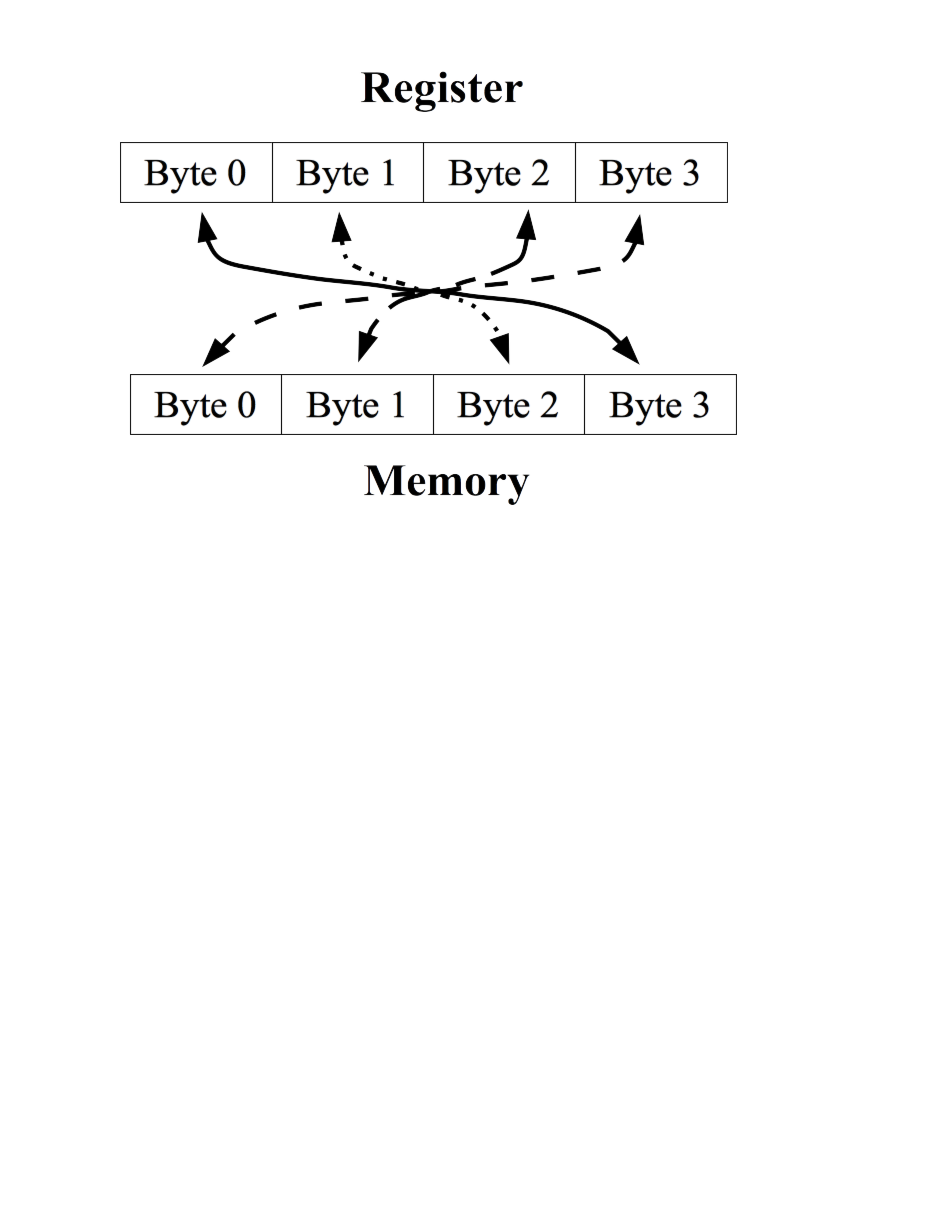
\includegraphics[width=\textwidth]{littleendian.png}
\end{figure}

Other processors are 
\emph{big-endian\index{big-endian}} processors, which means that they store 
the "big end", or most significant byte, of their words first, the way we would naturally read a number.

\begin{figure}
\caption{Register-to-memory transfers on big-endian systems}
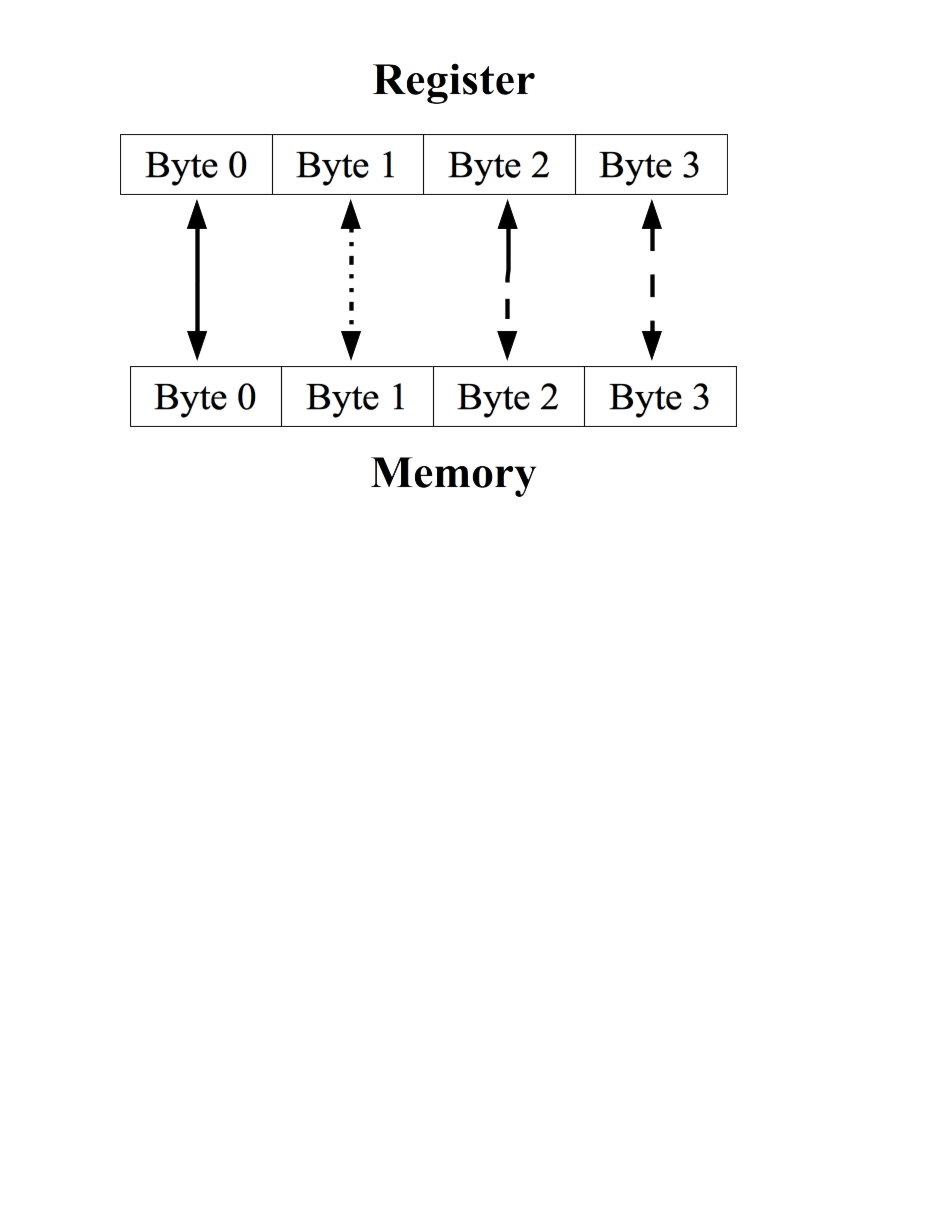
\includegraphics[width=\textwidth]{bigendian.png}
\end{figure}

This difference is not normally a problem (although it has sparked many
technical controversies throughout the years). 
Because the bytes are reversed again (or not, if it is a big-endian processor)
when being read back into a register\index{register}, the programmer usually never 
notices what order the bytes are in.  The byte-switching magic happens
automatically behind the scenes during register-to-memory transfers.  
However, the byte order can cause problems in several instances:

\begin{itemize}\item If you try to read in several bytes at a time using \icode{movl} but deal with them on a byte-by-byte basis using the least significant byte (i.e. - by using {\alReg} and/or shifting of the register), this will be in a different order than they appear in memory. 
\item If you read or write files written for different architectures, you may have to account for whatever order they write their bytes in. 
\item If you read or write to network sockets, you may have to account for a different byte order in the protocol. 
\end{itemize}

As long as you are aware of the issue, it usually isn't a big deal.  For more
in-depth look at byte order issues, you should read DAV's Endian FAQ at http://www.rdrop.com/~cary/html/endian\_faq.html, especially the article "On Holy Wars and a Plea for Peace" by Daniel Cohen.

\section{Converting Numbers for Display}

So far, we have been unable to display any number stored to the 
user, except by the extremely limitted means of passing it through
exit codes.  In this section, we will discuss converting positive numbers
into strings for display.

The function will be called \icode{integer2string}, and
it will take two parameters - an integer to convert and a string buffer 
filled with null characters (zeroes).  The buffer will be assumed to
be big enough to store the entire number as a string.(at least 11 characters
long, to include a trailing null character).

Remember that the way that we see numbers is in base 10.  Therefore, to access
the individual decimal digits of a number, we need to be dividing by 10
and displaying the remainder for each digit.  Therefore, the process will
look like this:

\begin{itemize}\item Divide the number by ten 
\item The remainder is the current digit.  Convert it to a character and store it. 
\item We are finished if the quotient is zero. 
\item Otherwise, take the quotient and the next location in the buffer and repeat the process. 
\end{itemize}

The only problem is that since this process deals with the one's place first,
it will leave the number backwards.  Therefore, we will have to finish by 
reversing the characters.  We will do this by storing the characters on
the stack as we compute them.  This way, as we pop them back off to fill
in the buffer, it will be in the reverse order that we pushed them on.

The code for the function should be put in a file called 
\icodefilename{integer-to-string.s} and should be entered as follows:

\begin{simpletyping}
\lstinputlisting{integer-to-string.s}
\end{simpletyping}

To show this used in a full program, use the following code, along
with the \icode{count\_chars} and \icode{write\_newline}
functions written about in previous chapters.  The code should be
in a file called \icodefilename{conversion-program.s}.

\begin{simpletyping}
\lstinputlisting{conversion-program.s}
\end{simpletyping}

To build the program, issue the following commands:

\begin{simpletyping}
\begin{lstlisting}
as integer-to-string.s -o integer-to-number.o
as count-chars.s -o count-chars.o
as write-newline.s -o write-newline.o
as conversion-program.s -o conversion-program.o
ld integer-to-number.o count-chars.o write-newline.o conversion-program.o -o conversion-program
\end{lstlisting}
\end{simpletyping}

To run just type \icode{./conversion-program} and the output
should say \icode{824}.

\section{Review}

\section{Know the Concepts}

\begin{itemize}\item Convert the decimal number 5,294 to binary. 
\item What number does 0x0234aeff represent?  Specify in binary, octal, and decimal. 
\item Add the binary numbers 10111001 and 101011. 
\item Multiply the binary numbers 1100 1010110. 
\item Convert the results of the previous two problems into decimal. 
\item Describe how AND, OR, NOT, and XOR work. 
\item What is masking for? 
\item What number would you use for the flags of the \icode{open} system call if you wanted to open the file for writing, and create the file if it doesn't exist? 
\item How would you represent -55 in a thirty-two bit register? 
\item Sign-extend the previous quantity into a 64-bit register. 
\item Describe the difference between little-endian and big-endian storage of words in memory. 
\end{itemize}

\section{Use the Concepts}

\begin{itemize}\item Go back to previous programs that returned numeric results through the exit status code, and rewrite them to print out the results instead using our integer to string conversion function. 
\item Modify the \icode{integer2string} code to return results in octal rather than decimal. 
\item Modify the \icode{integer2string} code so that the conversion base is a parameter rather than hardcoded. 
\item Write a function called \icode{is\_negative} that takes a single integer as a parameter and returns 1 if the parameter is negative, and 0 if the parameter is positive. 
\end{itemize}

\section{Going Further}

\begin{itemize}\item Modify the \icode{integer2string} code so that the conversion base can be greater than 10 (this requires you to use letters for numbers past 9). 
\item Create a function that does the reverse of \icode{integer2string} called \icode{number2integer} which takes a character string and converts it to a register-sized integer.  Test it by running that integer back through the \icode{integer2string} function and displaying the results. 
\item Write a program that stores likes and dislikes into a single machine word, and then compares two sets of likes and dislikes for commonalities. 
\item Write a program that reads a string of characters from STDIN and converts them to a number. 
\end{itemize}

